% =====================================================================
% Draft: Sections 2 (Materials and Methods) and 3 (Results and Discussion)
% for the summer-2026 ATLI rare-defect campaign.  REVISION 2 (2026-09-08).
%
% Structure follows Giovanny Vazquez's paper/thesis as the sample
% (per PI email). Section 1 (Introduction) and Related Work are
% PLACEHOLDERS for the PI; LaTeX renumbers automatically if Related
% Work is folded into the Introduction.
%
% Revision 2 integrates a three-agent review pass:
%  - PI-persona review: fixed mixup dose-sweep misattribution, family-
%    ordering claim, Jetson-table model mixing, fps/accuracy decoupling,
%    experiment-pool scoping, softened novelty claim, cut 5 tables.
%  - "Giovanny" style review: house takeaway phrasing, qualitative-figure
%    walkthrough (verified against the image), power-not-measured note,
%    poster figures swapped in (titles cropped for print).
%  - Citation agent: refs_sota.bib fully verified vs Crossref/arXiv/PMC.
% Every number traces to results/eval_eduardo_results.json,
% results/eval_v5obb_results.json, results/eval_blur_robustness.json,
% results/jetson_orin_nano_fps_benchmark.md, and results/*.md.
% Tables: mean +/- population std over 5 CV folds, in percent.
% =====================================================================
\documentclass[conference]{IEEEtran}
\usepackage{cite}
\usepackage{amsmath,amssymb}
\usepackage{graphicx}
\usepackage{booktabs}
\usepackage{multirow}
\usepackage{url}
\usepackage[caption=false,font=footnotesize]{subfig}

\newcommand{\dd}{Defective Damper}
\newcommand{\map}{mAP@0.5}

\begin{document}

\title{Data-Centric Rare-Defect Detection for Autonomous Transmission-Line Inspection with Lightweight Deep Learning Models\\
{\footnotesize (Working draft --- Sections II and III only; title, Introduction, and Related Work to be finalized by the PI)}}

\author{
\IEEEauthorblockN{Author List Pending}
\IEEEauthorblockA{Department of Electrical and Computer Engineering\\
University of Nevada, Las Vegas\\
Las Vegas, NV, USA}
}

\maketitle

\begin{abstract}
% Suggested headline claims kept for the GitHub record (all cross-validated):
% a data-centric training recipe (OBB, 1280 px, 3x defect oversampling,
% scale/rotation aug, mixup, blur aug) raises YOLO11n 66.8% -> 82.0% mAP@0.5
% and Defective Damper 50.1% -> 79.8% AP on the decontaminated 974-image
% benchmark, no external data, no architecture change; ordering holds across
% v5n/v8n/11n; 2.6M-param model ties 47M DINO-4scale on identical folds; every
% external-data route fails behind a leakage gate; Jetson Orin Nano 34.8 FPS
% @640 TensorRT FP16 (73-76%), or 82.0% @1280 at screening-rate 6.5-10.4 FPS.
[Placeholder. Potentially relevant citations: \cite{tsai2025atli,jocher2023ultralytics,zhang2023dino,vazquez2024wildfire,vazquez2026wildfire,zhang2018mixup}.]
\end{abstract}

\begin{IEEEkeywords}
transmission line inspection, defect detection, UAV, transfer learning, class imbalance, YOLO, oriented bounding boxes, edge computing
\end{IEEEkeywords}

% =====================================================================
\section{Introduction}
\textit{[To be written by the PI. Suggested anchors from the experimental side: U.S. outage statistics \cite{do2023outages}; UAV inspection reviews \cite{nguyen2018autonomous,liu2020review,yang2020powerline,faisal2025powerline}; the originating ATLI transfer-learning study \cite{tsai2025atli}; and the group's companion wildfire work \cite{vazquez2024wildfire,vazquez2026wildfire}, which this paper mirrors methodologically.]}

% =====================================================================
\section{Related Work}
\textit{[To be written by the PI. The bibliography files already contain the summer literature review (48+ entries): datasets \cite{tao2020insulator,shuang2023rsin,abdelfattah2020ttpla,vieiraesilva2021stnplad,oliveira2022furnas}, damper-specific detectors \cite{zhang2024dsanet,bao2021pmayolo,bao2022bcyolo,huang2023damper,liu2021slippage}, transformer detectors \cite{zhang2023padetr,zhang2024hcvit,carion2020detr}, and transfer learning in inspection \cite{shakiba2022insulator,pradeep2025insulator}. Verified 2025--2026 state-of-the-art references are collected in refs\_sota.bib with relevance notes (POLD-YOLO \cite{hu2026poldyolo}, CARE-Net \cite{zhou2026carenet}, PLD-DETR \cite{chen2025plddetr}, MLE-YOLOv11n \cite{wang2026mleyolo}, and the Drones 2026 survey \cite{fan2026survey}).]}

% =====================================================================
\section{Materials and Methods}
\label{sec:methods}

\subsection{Datasets Utilized}
\label{sec:datasets}
The target dataset of this work extends the Aerial Transmission Line Inspection (ATLI) dataset introduced in \cite{tsai2025atli}. ATLI contains 732 UAV and internet-sourced RGB images across seven categories---Birdnest, Broken Insulator, \dd{}, Flashover Insulator, Normal Damper, Normal Insulator, and Self-Exploded Insulator---and, unlike most public inspection datasets, annotates the defective \emph{spot} rather than the whole component. Two properties of this dataset motivate the present study. First, it is heavily imbalanced---a core open challenge of the field named in recent surveys \cite{faisal2025powerline,fan2026survey}: in the original ATLI, the rare, safety-critical \dd{} class has 113 instances against 1{,}460 Normal Dampers (${\sim}13{:}1$; ${\sim}9{:}1$ in the final benchmark of Table~\ref{tab:instances}). Second, a perceptual-hash (pHash) and filename audit revealed that three public datasets partially duplicate into the ATLI pool: 249 CPLID images \cite{tao2020insulator}, roughly half of a 300-image public sample of DVDI \cite{bao2022bcyolo}, and 32 PTL-AI Furnas evaluation images \cite{oliveira2022furnas}. External training data can therefore silently overlap the evaluation split. Dataset overlap takes two forms: literal duplicates (the same photograph, possibly re-encoded, resized, or cropped) and near-duplicate observations (the same scene captured from different viewpoints or zoom levels). The pHash-and-filename leakage gate applied to every dataset addition in this paper addresses the former; group-aware fold assignment (below) addresses the latter. All CPLID duplicates were removed from the benchmark.

The final benchmark merges the decontaminated extended ATLI pool (796 images) with 178 additional defect-focused images, for a total of 974 images. The additional images were hand-selected by the authors from the 10{,}698-image in-domain inspection pool described below, prioritizing images that contain the rare defect classes---defective dampers and defective insulators---with an emphasis on zoomed-out views, in contrast to the close-range framing of datasets such as CPLID \cite{tao2020insulator}. They were re-annotated in Roboflow with the ATLI defect-spot taxonomy, verified to share no images with the ATLI pool, and reduced from an initial 300 to 178 by exact- and near-duplicate removal under the same pHash gate. All images are $640^2$ or $512^2$ pixels. The pool is divided with a 70/15/15 train/validation/test ratio into five stratified cross-validation folds with disjoint test splits; because the added images retain 21 clusters of near-duplicate views of the same scenes, fold assignment is group-aware, keeping each cluster within a single split. Table~\ref{tab:instances} lists the per-class instance counts. Oversampling and augmentation (Section~\ref{sec:learning}) are applied to training splits only; validation and test splits are never modified.

\begin{table}[t]
\caption{Instance counts of the 974-image benchmark. Train/validation/test columns are per-fold means over the five cross-validation folds; OS = the $3\times$ defect-class oversampling of Section~\ref{sec:learning}.}
\label{tab:instances}
\centering
\footnotesize
\setlength{\tabcolsep}{3.5pt}
\begin{tabular}{lrrrrr}
\toprule
Class & Total & Train & Train (OS) & Val. & Test \\
\midrule
Birdnest & 234 & 163 & 173 & 35 & 36 \\
Broken Insulator & 290 & 206 & 618 & 40 & 44 \\
\dd{} & 193 & 134 & 401 & 30 & 29 \\
Flashover Insulator & 433 & 303 & 910 & 65 & 65 \\
Normal Damper & 1714 & 1208 & 2321 & 248 & 258 \\
Normal Insulator & 1457 & 1037 & 2171 & 211 & 209 \\
Self-Exploded Insulator & 304 & 207 & 622 & 47 & 50 \\
\midrule
Images & 974 & 683 & 1647 & 146 & 145 \\
\bottomrule
\end{tabular}
\end{table}

Four auxiliary image sources are used. (i) The Microsoft COCO dataset \cite{lin2014coco} serves as the heterogeneous source dataset for transfer learning, following \cite{tsai2025atli,vazquez2024wildfire}. (ii) An external damper pool of 2{,}175 images (1{,}430 containing defective dampers), assembled from two public Roboflow Universe datasets \cite{wangbo2025damper,yolov11tasks2025damper} and passed through the leakage gate, is used for the external-data experiments. (iii) A 10{,}698-image in-domain inspection pool with generic component labels serves both as the selection pool for the 178 added benchmark images (above) and as the source for the in-domain pretraining experiments; it aggregates public inspection datasets (including STN PLAD \cite{vieiraesilva2021stnplad} and, before decontamination, CPLID \cite{tao2020insulator}), Roboflow Universe community datasets, and web-collected UAV imagery. (iv) The 249 removed CPLID images are used in a controlled train-only restoration experiment. Test splits are always kept clean of CPLID, both to preserve the leakage-free protocol and because CPLID's defective-insulator images are synthetically composited \cite{tao2020insulator}; augmented imagery in the evaluation split would not reflect the field conditions an edge-deployed inspection system encounters, whereas it remains a legitimate training resource. An earlier phase of the campaign, predating the decontamination, used a 1{,}343-image merged pool; the comparison against heavyweight state-of-the-art detectors (Section~\ref{sec:sota}) and the external-data study (Section~\ref{sec:external}) were conducted on that pool and are scoped accordingly.

\subsection{Experiment Setup}
Table~\ref{tab:platforms} describes the GPU server used for all training and the edge computing device used for the deployment evaluation. Heavyweight baseline detectors are trained with MMDetection 3.3.0 \cite{chen2019mmdetection} on the same server.

\begin{table}[t]
\caption{Experimental platform configurations.}
\label{tab:platforms}
\centering
\footnotesize
\setlength{\tabcolsep}{4pt}
\begin{tabular}{lll}
\toprule
 & GPU Server & Edge Device \\
\midrule
Hardware & Quadro RTX 6000 24\,GB $\times$ 8 & Jetson Orin Nano (15\,W) \\
CPU & Intel Xeon Gold 5218 & Arm Cortex-A78AE \\
Environment & Python 3.10 & Python 3.12, JetPack 7.2 \\
Framework & PyTorch 2.6, Ultralytics 8.4 \cite{jocher2023ultralytics} & PyTorch 2.13 \\
Computing & CUDA 11.8 & CUDA 13.2, TensorRT 11.1 \\
\bottomrule
\end{tabular}
\end{table}

\subsection{Model Selection}
\label{sec:models}
Lightweight YOLO architectures have repeatedly been shown to provide a strong speed--accuracy trade-off for transmission-line inspection \cite{tsai2025atli,faisal2025powerline} and for the group's companion UAV wildfire work \cite{vazquez2024wildfire,vazquez2026wildfire}. Within the set of existing YOLO architectures, the Ultralytics nano variants \cite{jocher2023ultralytics} are selected for being low-weight, high-performing models directly comparable to the original ATLI study \cite{tsai2025atli}: YOLOv5n (2.51M parameters, 7.2 GFLOPs at 640\,px), YOLOv8n (3.08M, 8.5), and YOLO11n (2.66M, 6.7). Each model is trained in two task modes: standard axis-aligned detection, and oriented-bounding-box (OBB) detection, in which the network additionally regresses a rotation angle and boxes are minimum-area rotated rectangles. OBB labels are generated from the benchmark's polygon annotations via minimum-area-rectangle conversion. Ultralytics provides no OBB variant of YOLOv5n; for completeness, the YOLOv5 OBB configuration is trained on a community YOLOv5-OBB fork and evaluated with the DOTA rotated-box protocol \cite{xia2018dota}, and is marked accordingly wherever it appears.

% TODO(citation): the Ghost ~8-mAP / 4x-CPU-speedup result and the graft-methodology credit currently cite vazquez2026wildfire, but that result is in the Vazquez thesis ("(c) 2025 IEEE" tables), not the published Sensors paper -- confirm the correct IEEE target with Giovanny/the PI (citation_audit.md, issue 1). Same citation is used in Sec. IV-F.
To test whether accuracy gains require heavier architectures, three state-of-the-art detectors spanning the main design families are selected from MMDetection \cite{chen2019mmdetection}: DINO-4scale \cite{zhang2023dino} (transformer, ResNet-50, 47M parameters), RTMDet-Tiny \cite{lyu2022rtmdet} (one-stage, 4.8M), and Dynamic R-CNN \cite{zhang2020dynamicrcnn} (two-stage, ResNet-50-FPN, 41M), all COCO-pretrained and trained at their default configurations, standard epoch budgets, and default input resolutions (${\sim}1333{\times}800$ for DINO and Dynamic R-CNN, $640^2$ for RTMDet). In the opposite direction, three lightweight backbone replacements (2.18--2.84M parameters) are grafted onto the nano models to test whether the models can be made \emph{smaller} without accuracy loss: GhostNet modules \cite{han2020ghostnet}, depthwise-separable convolutions (DWS) \cite{howard2017mobilenets}, and FasterNet partial convolutions \cite{chen2023fasternet}, mirroring the optimization methodology of \cite{vazquez2026wildfire}; a P2 model variant, which adds an extra detection head on the high-resolution stride-4 feature map to improve small-object detection, is also evaluated. Parameter counts and GFLOPs are reported as descriptive quantities only: as Section~\ref{sec:edge} shows, they are poor predictors of deployed throughput---batch-1 inference is launch-overhead-bound on datacenter GPUs, and on the edge device TensorRT's kernel-level optimization of standard convolutions means nominally lighter operators are not reliably faster---so all speed claims in this paper rest on on-device measurement rather than complexity proxies.

\subsection{Learning Methods}
\label{sec:learning}
All YOLO models are trained with a two-stage transfer-learning procedure derived from \cite{tsai2025atli}: the model is initialized from the published COCO-pretrained checkpoint, trained on the target data for 150 epochs (stage one), and then fine-tuned for 100 additional epochs with all layers unfrozen at a much lower learning rate (stage two). This is the three-stage procedure of \cite{tsai2025atli} with its first stage---training the source model on COCO---replaced by the published checkpoint, and with the fine-tuning stage matching that study's best configuration (all layers unfrozen). Table~\ref{tab:hyper} lists the hyperparameter settings; all hyperparameters not explicitly mentioned are left at the Ultralytics defaults, so the default augmentation pipeline (mosaic, HSV jitter, flips) is active in every run, including the baseline.

\begin{table}[t]
\caption{Training hyperparameter settings.}
\label{tab:hyper}
\centering
\footnotesize
\begin{tabular}{ll}
\toprule
Hyperparameter & Value \\
\midrule
Optimizer & SGD \\
Stage-one epochs / initial LR & 150 / 0.01 \\
Stage-two epochs / initial LR & 100 / 0.00334 \\
Stage-two final LR fraction & 0.1535 (one-cycle) \\
Batch size & 16 \\
Input image size & 640 or 1280 (per condition) \\
Layers frozen & 0 \\
\bottomrule
\end{tabular}
\end{table}

The following training techniques were tested:
\begin{enumerate}
\item \textbf{High-resolution training} (1280\,px): counteracts the small pixel footprint of defective components.
\item \textbf{Defect-class oversampling} ($3\times$): every training image containing any of the four defect classes is duplicated three times; online augmentation gives each copy a distinct view. Training splits only.
\item \textbf{Scale augmentation} (scale jitter 0.9): exposes the model to smaller object views.
\item \textbf{OBB task mode}: rotated boxes fit elongated components tightly and make rotation augmentation geometrically consistent.
\item \textbf{Rotation augmentation} ($\pm15^\circ$ to $\pm30^\circ$): evaluated under both task modes; an angle sweep ($15^\circ$--$45^\circ$) locates the useful range.
\item \textbf{Mixup} (ratio 0.15) \cite{zhang2018mixup}: overlays two training images and combines their labels, which regularizes the model; ratios 0.10--0.25 were swept.
\item \textbf{Blur augmentation}: motion blur ($p{=}0.3$) and Gaussian blur ($p{=}0.2$) applied through the Albumentations pipeline \cite{buslaev2020albumentations} to simulate UAV camera motion blur.
\end{enumerate}
These techniques are evaluated in Table~\ref{tab:ladderres} through incremental technique addition: each row adds one technique to the configuration above it, so consecutive rows isolate the added technique's contribution; dose sweeps and rejected variants are reported in Sections~\ref{sec:ladder} and~\ref{sec:ablations}.

The techniques above help address the rare-class bottleneck by better using the existing data. The alternative is to add external defect data. To test it, four routes to ``more defect data'' are evaluated: direct mixing of the external damper pool into training at doses from 1:1 to 11.7:1 (normal-to-defective instance ratio); scale-matched curation restricted to the native object-size distribution; pretraining on the external pool followed by fine-tuning on native data; and in-domain source pretraining on the 10{,}698-image inspection pool in place of COCO. Two controls localize any failure: a model trained and evaluated entirely within the external distribution (tests whether the external labels are learnable at all), and a leakage-checked bird-nest dataset addition (tests what a healthy external addition looks like). Finally, the 249 removed CPLID images are restored to training only, on top of the strongest recipes, to test whether curated public data composes with the data-centric techniques.

\subsection{Evaluation Metrics}
\label{sec:metrics}
Two key metrics are used to measure detection accuracy: Average Precision (AP) per class and mean Average Precision (mAP). These depend on Precision and Recall, defined in \eqref{eq:prec} and \eqref{eq:rec}, where TP, FP, and FN represent true positives, false positives, and false negatives for a given class, respectively:
\begin{equation}
\label{eq:prec}
\text{Precision} = \frac{TP}{TP + FP},
\end{equation}
\begin{equation}
\label{eq:rec}
\text{Recall} = \frac{TP}{TP + FN}.
\end{equation}
A prediction counts as a true positive when its box overlaps a ground-truth box of the same class with Intersection over Union (IoU), defined in \eqref{eq:iou}, at or above a threshold:
\begin{equation}
\label{eq:iou}
\text{IoU} = \frac{\mathit{area}(\text{ground truth} \cap \text{prediction})}{\mathit{area}(\text{ground truth} \cup \text{prediction})}.
\end{equation}
AP is the area under the precision--recall curve, and mAP averages AP over the $k{=}7$ classes:
\begin{equation}
\label{eq:ap}
AP = \int_0^1 p(r)\,dr,
\end{equation}
\begin{equation}
\label{eq:map}
mAP = \frac{1}{k}\sum_{i=1}^{k} AP_i.
\end{equation}
For this study the IoU threshold is 0.5 (\map{}). Recall is reported at the F1-optimal confidence threshold. For OBB models, IoU is computed between rotated boxes; the YOLOv5-OBB fork is scored with the DOTA Task-1 rotated-box protocol \cite{xia2018dota}.

Because the rare \dd{} class has only ${\sim}29$ test instances per fold, single-split per-class AP is extremely noisy, so all results are reported as the mean $\pm$ standard deviation over the five cross-validation folds. Validation splits serve only for checkpoint selection, and test splits are touched once per run; unlike \cite{vazquez2024wildfire,vazquez2026wildfire}, validation accuracies are therefore not tabulated. On the edge device, inference speed is measured as end-to-end batch-1 frames per second (FPS)---preprocessing, forward pass, and non-maximum suppression or OBB decoding---with clocks pinned at the maximum 15\,W profile, for PyTorch FP32, TensorRT FP16, and TensorRT INT8 (entropy-calibrated on one validation fold) export formats. Following \cite{vazquez2026wildfire}, 25--30 FPS is treated as the real-time standard for drone footage, while a coverage analysis of line-following flight indicates 5--10 FPS suffices for still-image screening.

% =====================================================================
\section{Results and Discussion}
\label{sec:results}

To evaluate the data-centric training methodology, the following experiments have been conducted:
\begin{enumerate}
\item incremental evaluation of the training recipe;
\item per-class analysis of the resulting final recipe;
\item comparison of lightweight YOLO versions;
\item comparison with heavyweight state-of-the-art models;
\item evaluation of external-data alternatives;
\item ablations and negative results, including lighter backbones;
\item resolution scaling and measured edge deployment.
\end{enumerate}
Experiments (4) and (5) were produced on the earlier 1{,}343-image pool (Section~\ref{sec:datasets}); experiment (7) was produced on the edge computing device; all other results were produced by the GPU server on the 974-image benchmark.

\subsection{Incremental Training-Recipe Results}
\label{sec:ladder}
Table~\ref{tab:ladderres} reports the incremental recipe results on YOLO11n. The full recipe raises \map{} from 66.8\% to 82.0\% ($+15.2$ points) and raises the rare \dd{} class from 50.1\% to 79.8\% AP ($+29.7$ points), with \dd{} recall---the safety-critical metric---rising from 44.6\% to 72.0\%.

\begin{table}[t]
\caption{Incremental recipe results on the 974-image benchmark (YOLO11n, mean $\pm$ std over 5 folds). Each row adds one technique to the row above it. Best per column in bold.}
\label{tab:ladderres}
\centering
\scriptsize
\setlength{\tabcolsep}{3.5pt}
\begin{tabular}{lccc}
\toprule
Configuration & \map{} (\%) & DD AP (\%) & DD Recall (\%) \\
\midrule
Baseline (640, detect) & $66.8 \pm 4.3$ & $50.1 \pm 15.6$ & $44.6$ \\
+ OS, 1280, scale (detect) & $74.9 \pm 3.8$ & $61.7 \pm 15.6$ & $57.7$ \\
+ OBB & $75.9 \pm 1.9$ & $67.2 \pm 9.5$ & $65.7$ \\
+ rotation ($15^\circ$) & $79.3 \pm 2.3$ & $72.9 \pm 9.6$ & $67.1$ \\
+ mixup (0.15) & $80.4 \pm 1.9$ & $76.0 \pm 10.4$ & $66.1$ \\
+ blur, deg30 (final recipe) & $\mathbf{82.0 \pm 2.2}$ & $\mathbf{79.8 \pm 10.8}$ & $\mathbf{72.0}$ \\
\bottomrule
\multicolumn{4}{l}{DD = \dd{}; OS = $3\times$ defect oversampling.}
\end{tabular}
\end{table}

These results provide four key takeaways. First, the largest single step is the combination of resolution, oversampling, and scale augmentation ($+8.1$ mAP): the rare-class bottleneck is primarily a small-object and under-exposure problem, not a modeling problem. The OBB step adds another point; since rotated-box and axis-aligned mAP are not the identical measurement, a detection-mode control on identical folds of the earlier pool was run and showed task mode itself is a wash overall, with OBB's benefit concentrated in box tightness on elongated components. Second, rotation augmentation helps only in OBB mode, where the box rotates with the object. The angle sweep puts the sweet spot near $15^\circ$ (79.3\%), flat through $30^\circ$, and collapsed at $\pm45^\circ$ (75.8\%). Under axis-aligned detection the same augmentation hurts (a $10^\circ$ rotation costs 10 \dd{} AP points), even though rotation is applied uncritically in much of the inspection literature. Third, the techniques do not compose freely: on top of the $15^\circ$ rotation configuration, restoring CPLID training data (79.2\%), adding shear (78.8\%), and adding blur augmentation (79.0\%) all failed to improve \map{}. Mixup is the exception---as a photometric regularizer rather than a geometric transform, it adds $+1.1$ mAP on top of rotation; a dose sweep at 640\,px shows a plateau between 0.15 and 0.25 (75.7\% vs.\ 75.9\%) with a drop at 0.10 (73.9\%). Lastly, blur augmentation and mixup together unlock a stronger rotation dose: with both active, $\pm30^\circ$ becomes the best configuration (82.0\%), even though $30^\circ$ alone is not better than $15^\circ$ and blur alone is neutral. The final recipe is an interaction effect, not a sum of independent gains. Prior inspection work applies such augmentations only inside undifferentiated stacks (e.g., mixup in \cite{farooq2026teyolov8}); to the best of the authors' knowledge, this is the first work to isolate their individual contributions under cross-validation, and oriented bounding boxes remain rare in this application domain.

\subsection{Per-Class Performance of the Final Recipe}
Table~\ref{tab:perclass} compares the baseline and final-recipe models class by class, and Fig.~\ref{fig:qual} shows inference results on five test scenarios: a distribution pole with multiple defective dampers, a close-up broken-insulator string, a self-exploded insulator on a lattice tower, a hillside tower with mixed components, and a nest-bearing tower against vegetation. The following observations are noted. In column one, the final recipe recovers additional defective dampers, including one the baseline labels Normal Damper. In column two, the baseline detects nothing while the final recipe finds all four broken shells (confidence 0.44--0.67). Column three shows both models detecting the self-exploded insulator, with the rotated boxes fitting the elongated strings more tightly. In column four the final recipe adds a birdnest missed by the baseline. Lastly, in column five, the baseline triple-detects the same nest at low confidence (0.28--0.59) while the final recipe produces a single detection at 0.86. Overall, the gains concentrate on small defects and duplicate suppression.

Every class improves, and the four defect classes improve the most ($+15$ to $+30$ AP points): the recipe's gains land where the inspection task needs them. Error analysis of the baseline shows that defect classes are rarely \emph{confused} with their normal counterparts; their dominant failure mode is missed detection of small defects, which is precisely the failure mode that resolution, oversampling, and scale augmentation attack. This also explains why detect-then-classify architectures, proposed elsewhere for visually similar defect pairs \cite{zhang2023padetr,souza2023hybridyolo}, address a confusion this benchmark mostly does not exhibit. For context, damper defects are the worst or near-worst class in every multi-class study reviewed (63.6\% AP in \cite{zhang2024dsanet}, 40.0\% in \cite{su2024cessd}), and recent damper-condition detectors report only on custom single-purpose datasets \cite{zhou2026carenet}. The cross-validated 79.8\% here, from a stock architecture, sits at the favorable end of these results, though datasets differ and direct comparison is not possible.

\begin{table}[t]
\caption{Per-class AP@0.5 (\%, mean $\pm$ std over 5 folds) and recall (\%) of baseline vs.\ final recipe (YOLO11n).}
\label{tab:perclass}
\centering
\scriptsize
\setlength{\tabcolsep}{3pt}
\begin{tabular}{lcccc}
\toprule
 & \multicolumn{2}{c}{Baseline} & \multicolumn{2}{c}{Final recipe} \\
\cmidrule(lr){2-3}\cmidrule(lr){4-5}
Class & AP & R & AP & R \\
\midrule
Birdnest & $92.2 \pm 2.0$ & 88.3 & $94.6 \pm 2.1$ & 92.2 \\
Broken Insulator & $57.4 \pm 6.8$ & 53.2 & $77.2 \pm 7.5$ & 70.6 \\
\dd{} & $50.1 \pm 15.6$ & 44.6 & $79.8 \pm 10.8$ & 72.0 \\
Flashover Insulator & $59.6 \pm 6.3$ & 52.7 & $74.5 \pm 6.1$ & 68.3 \\
Normal Damper & $66.2 \pm 4.2$ & 57.3 & $78.8 \pm 3.1$ & 75.3 \\
Normal Insulator & $78.9 \pm 3.7$ & 76.6 & $84.6 \pm 3.3$ & 83.1 \\
Self-Exploded Insulator & $63.2 \pm 6.0$ & 53.1 & $84.5 \pm 5.5$ & 80.4 \\
\midrule
Overall & $66.8 \pm 4.3$ & 60.9 & $82.0 \pm 2.2$ & 77.4 \\
\bottomrule
\end{tabular}
\end{table}

\begin{figure}[t]
\centering
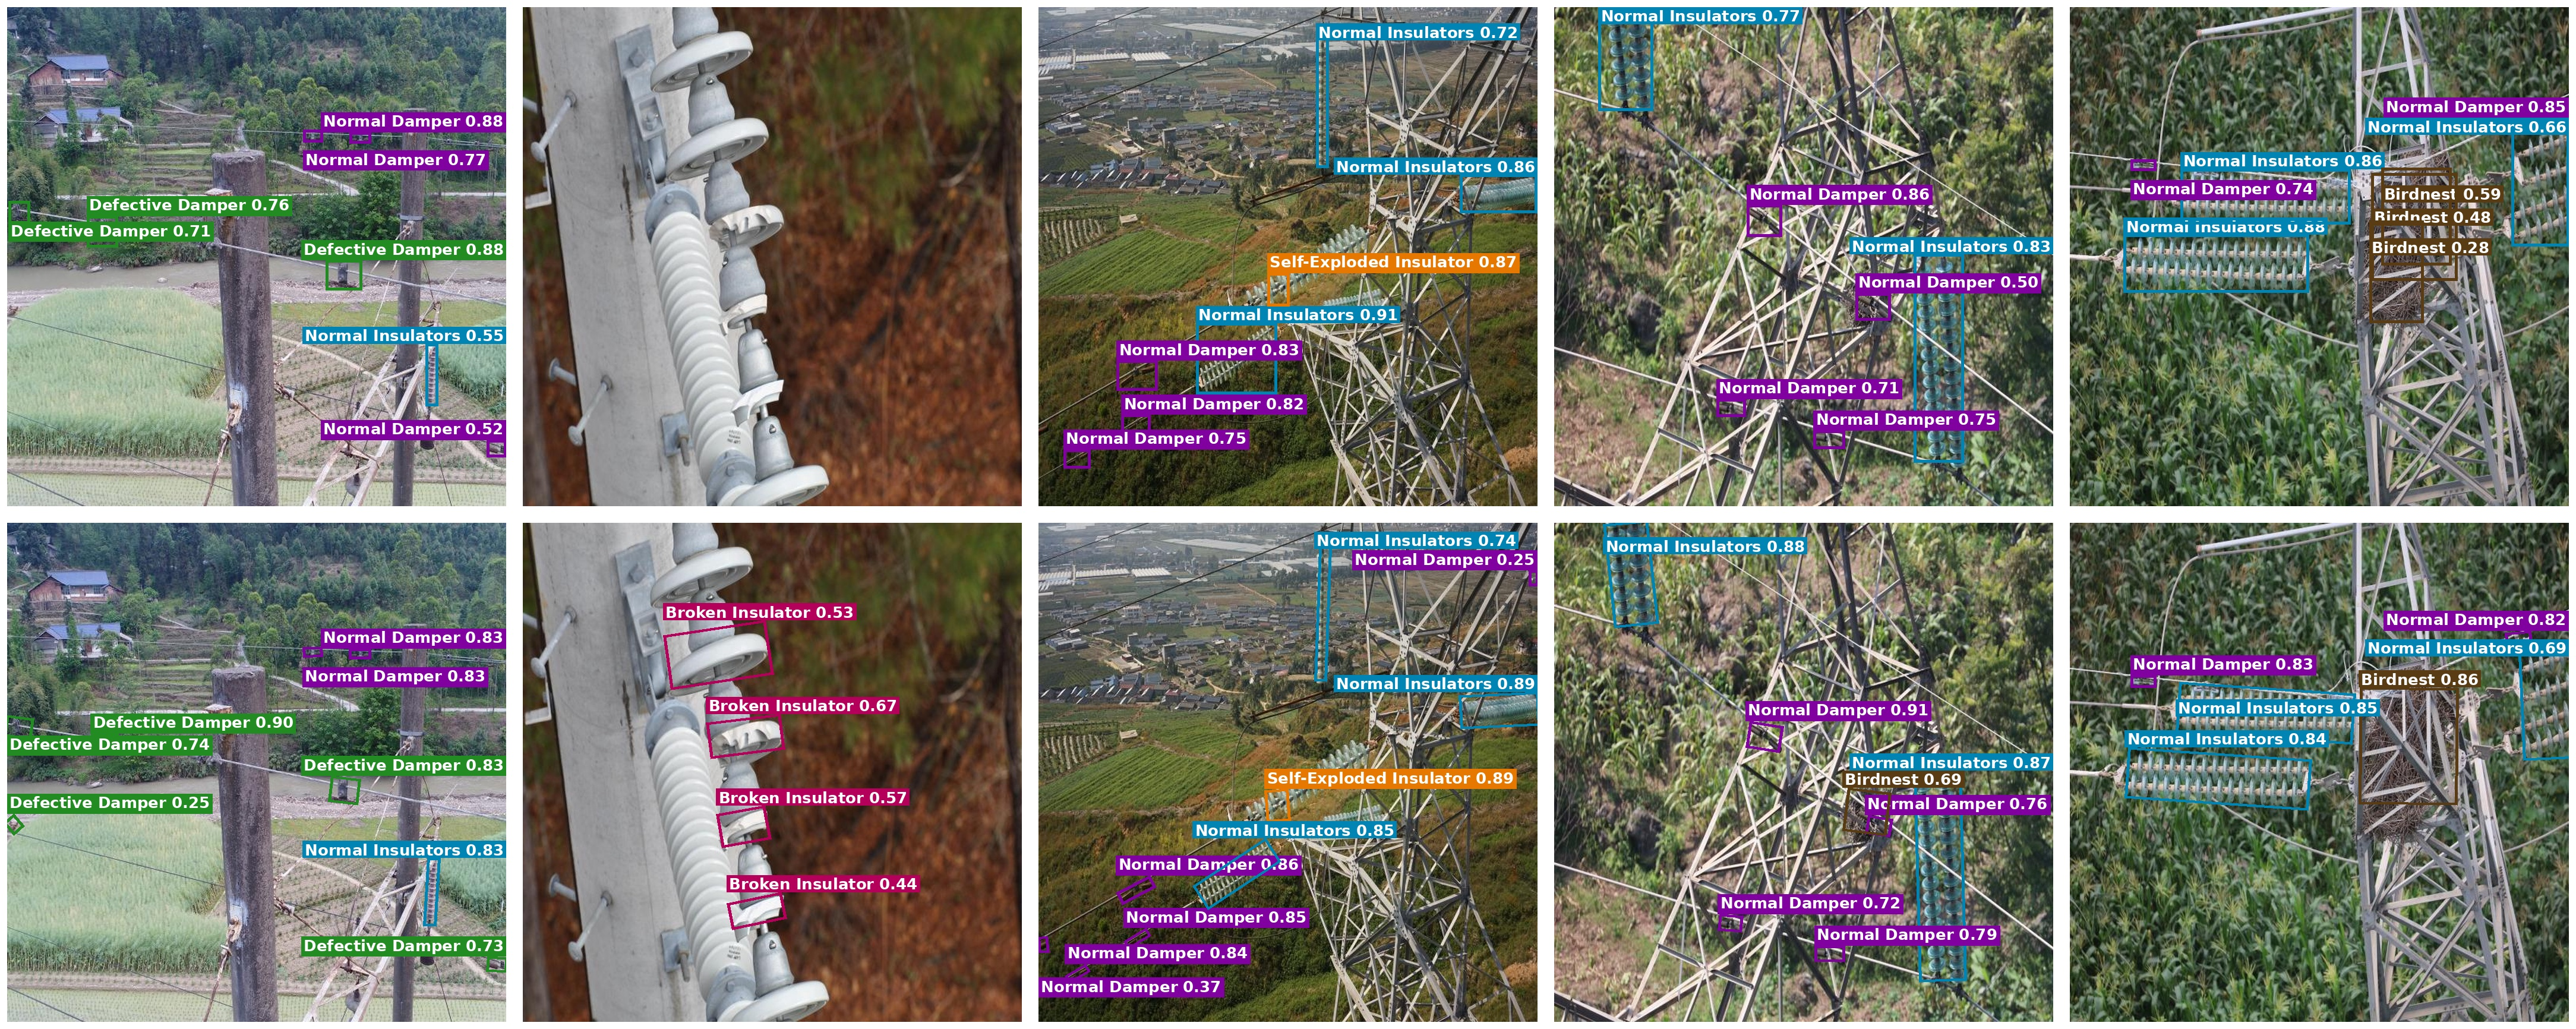
\includegraphics[width=\columnwidth]{figures/fig_obb_before_after.jpg}
\caption{Comparison of inference results on five test scenarios: baseline (top) vs.\ final recipe (bottom). From left to right, columns 1--5.}
\label{fig:qual}
\end{figure}

\subsection{Comparison of Lightweight YOLO Versions}
\label{sec:family}
Fig.~\ref{fig:ladderfig} applies the same incremental recipe to YOLOv5n and YOLOv8n on identical folds. These results provide three key takeaways. First, the recipe ordering is architecture-independent: every technique that helps YOLO11n also helps YOLOv8n and (where applicable) YOLOv5n, so the data-centric findings transfer across the model family. Second, YOLO11n leads at the two strongest configurations (79.3\% and 80.4\%); YOLOv8n overtakes it at the plain OBB configuration (76.5\% vs.\ 75.9\%) and closes to within 0.6 points with mixup (79.8\%); YOLOv5n is competitive in detection mode but cannot follow the recipe past OBB. Lastly, YOLOv5n is the only model whose OBB configuration \emph{loses} to its detection configuration (67.1\%* vs.\ 73.1\%)---but since it could only be run on a community fork under a slightly different evaluation protocol, this result carries an asterisk and no strong conclusion is drawn from it.

\begin{figure}[t]
\centering
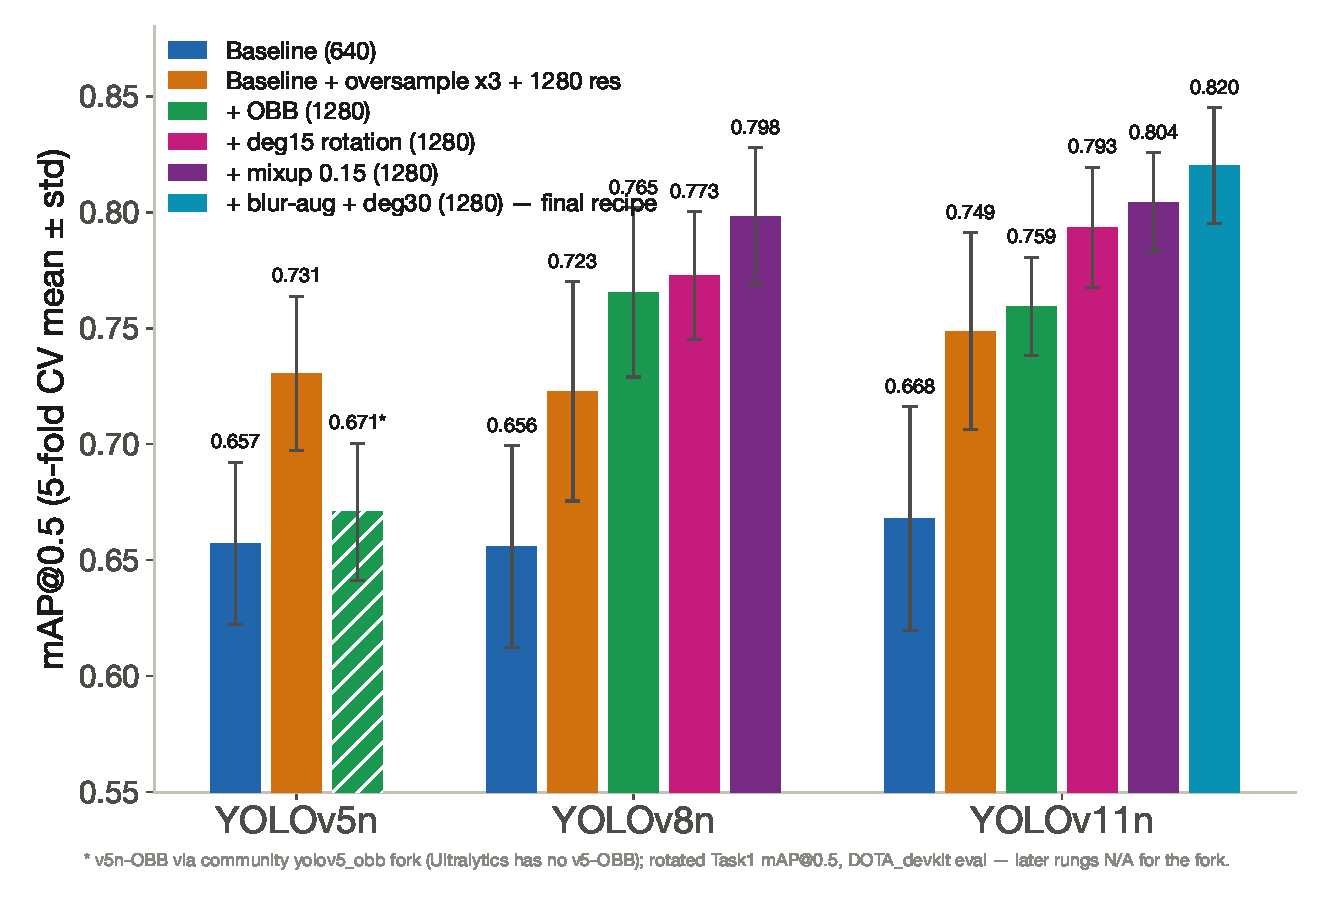
\includegraphics[width=\columnwidth]{figures/fig_ladder_paper.pdf}
\caption{Incremental recipe results across the YOLO nano family (\map{}, 5-fold cross-validation mean $\pm$ std). Hatched bar (*): YOLOv5-OBB community fork scored with the DOTA rotated protocol \cite{xia2018dota}, not directly comparable; later recipe steps are unavailable for the fork.}
\label{fig:ladderfig}
\end{figure}

\subsection{Comparison with State-of-the-Art Models}
\label{sec:sota}
Table~\ref{tab:sota} compares the tuned nano recipe with the three MMDetection baselines. This experiment used the earlier 1{,}343-image pool under the same five-fold protocol; the recipe at that stage was 1280\,px + oversampling + scale, detection mode. The heavyweights run at stock configurations, so this measures a tuned nano against off-the-shelf heavyweights, not their ceiling. Under that scoping, the 2.6M-parameter YOLO11n recipe ties the 47M-parameter DINO-4scale on \map{} (78.5\% both) with lower fold variance, and is comparable on the rare class (81.2\% vs.\ 78.9\%; paired per-fold difference $+2.3 \pm 5.0$ points, within fold noise) at ${\sim}18\times$ fewer parameters. RTMDet-Tiny, the closest efficiency rival at 4.8M parameters, trails by 3.8 mAP points, a deficit positive on all five folds. The tuned recipe also exceeds the originating study's best YOLOv11n transfer-learning result under this stricter evaluation (78.5\% vs.\ 76.8\% \cite{tsai2025atli}). Notably, all three heavyweights score 3--6 points \emph{higher} under cross-validation than on the original fixed split, confirming that single-split evaluation on datasets of this size is a pessimistic and noisy draw even for large models. Applying the same data-centric techniques to a heavyweight is future work; the narrower claim is that on a small inspection benchmark, parameter count buys no accuracy premium over disciplined data-centric training of a nano model.

\begin{table}[t]
\caption{Comparison with state-of-the-art models on identical 5-fold splits of the earlier 1{,}343-image pool (MMDetection defaults, COCO-pretrained).}
\label{tab:sota}
\centering
\scriptsize
\setlength{\tabcolsep}{3pt}
\begin{tabular}{lcccc}
\toprule
Model & Params (M) & Epochs & \map{} (\%) & DD AP (\%) \\
\midrule
DINO-4scale \cite{zhang2023dino} & 47 & 36 & $\mathbf{78.5 \pm 3.2}$ & $78.9 \pm 11.0$ \\
RTMDet-Tiny \cite{lyu2022rtmdet} & 4.8 & 150 & $74.7 \pm 2.3$ & $77.4 \pm 5.2$ \\
Dynamic R-CNN \cite{zhang2020dynamicrcnn} & 41 & 40 & $71.8 \pm 2.3$ & $69.9 \pm 6.5$ \\
\midrule
YOLO11n baseline & \textbf{2.6} & 150+100 & $72.2 \pm 1.9$ & $74.3 \pm 7.4$ \\
YOLO11n tuned recipe & \textbf{2.6} & 150+100 & $\mathbf{78.5 \pm 2.3}$ & $\mathbf{81.2 \pm 8.0}$ \\
\bottomrule
\multicolumn{5}{l}{DD = \dd{}.}
\end{tabular}
\end{table}

\subsection{External-Data Alternatives: A Systematic Negative Result}
\label{sec:external}
The intuitive alternative to the data-centric recipe---harvesting more defective-damper data---was evaluated exhaustively on the earlier pool's fixed split (seed-averaged; baseline \dd{} AP $64.1 \pm 3.6$\% over 11 seeds). Every route failed. Direct mixing of the leakage-gated external pool never beat the baseline at any dose from 1:1 to 11.7:1 ($n{=}8$); scale-matched curation performed no better ($n{=}3$) while dropping \dd{} recall to 51\%; no pretrain-then-finetune schedule improved on the baseline; and in-domain source pretraining on the 10{,}698-image inspection pool, evaluated under the decontaminated single-split protocol, produced genuine \emph{negative} transfer ($-7.5$ mAP versus COCO initialization). The same failure held for the different models tested (YOLOv5n and YOLOv8n). Two controls localize it: a model trained and evaluated within the external distribution reaches ${\approx}91\%$ \dd{} AP---the external labels are perfectly learnable---and the healthy bird-nest addition ($n{=}1$) lifted its own target class by $+13.6$ points.

External damper data does not fail because it is bad data. Its notion of ``defective'' and its capture distribution do not match the target's; the signature is a recall drop at held precision. A recent domain-generalization study reports the same cross-domain loss for damper-defect detectors \cite{yang2025oneforall}, and synthetic-defect generation is emerging precisely because harvested real data transfers poorly \cite{stefenon2026diffusion}. The group's wildfire result is the mirror image: a curated source sharing the target's label semantics beat COCO by 14.4 mAP \cite{vazquez2024wildfire,vazquez2026wildfire}. What transfers is label-style consistency, not domain proximity.

The controlled CPLID restoration completes the picture on the current benchmark: restoring the 249 curated CPLID images to training only lifts the mixup configuration slightly (80.4\%$\to$81.1\%, with \dd{} recall $+8.8$ points) but fails to improve the final recipe (82.0\%$\to$81.3\%). Curated public data helps weaker configurations and washes out on the strongest one---the same composition ceiling observed among the augmentation techniques. The practical guidance: on small inspection benchmarks, exhaust native data-centric techniques before harvesting external data, and never harvest without a leakage gate (Section~\ref{sec:datasets}).

% Negative-results figure removed from the paper (2026-09-10) — kept here as a
% comment for the GitHub record; the paragraph above states all of its numbers.
% Source figure: figures/fig_external_paper.pdf (generator: paper/poster/figs_src/).
%\begin{figure*}[t]
%\centering
%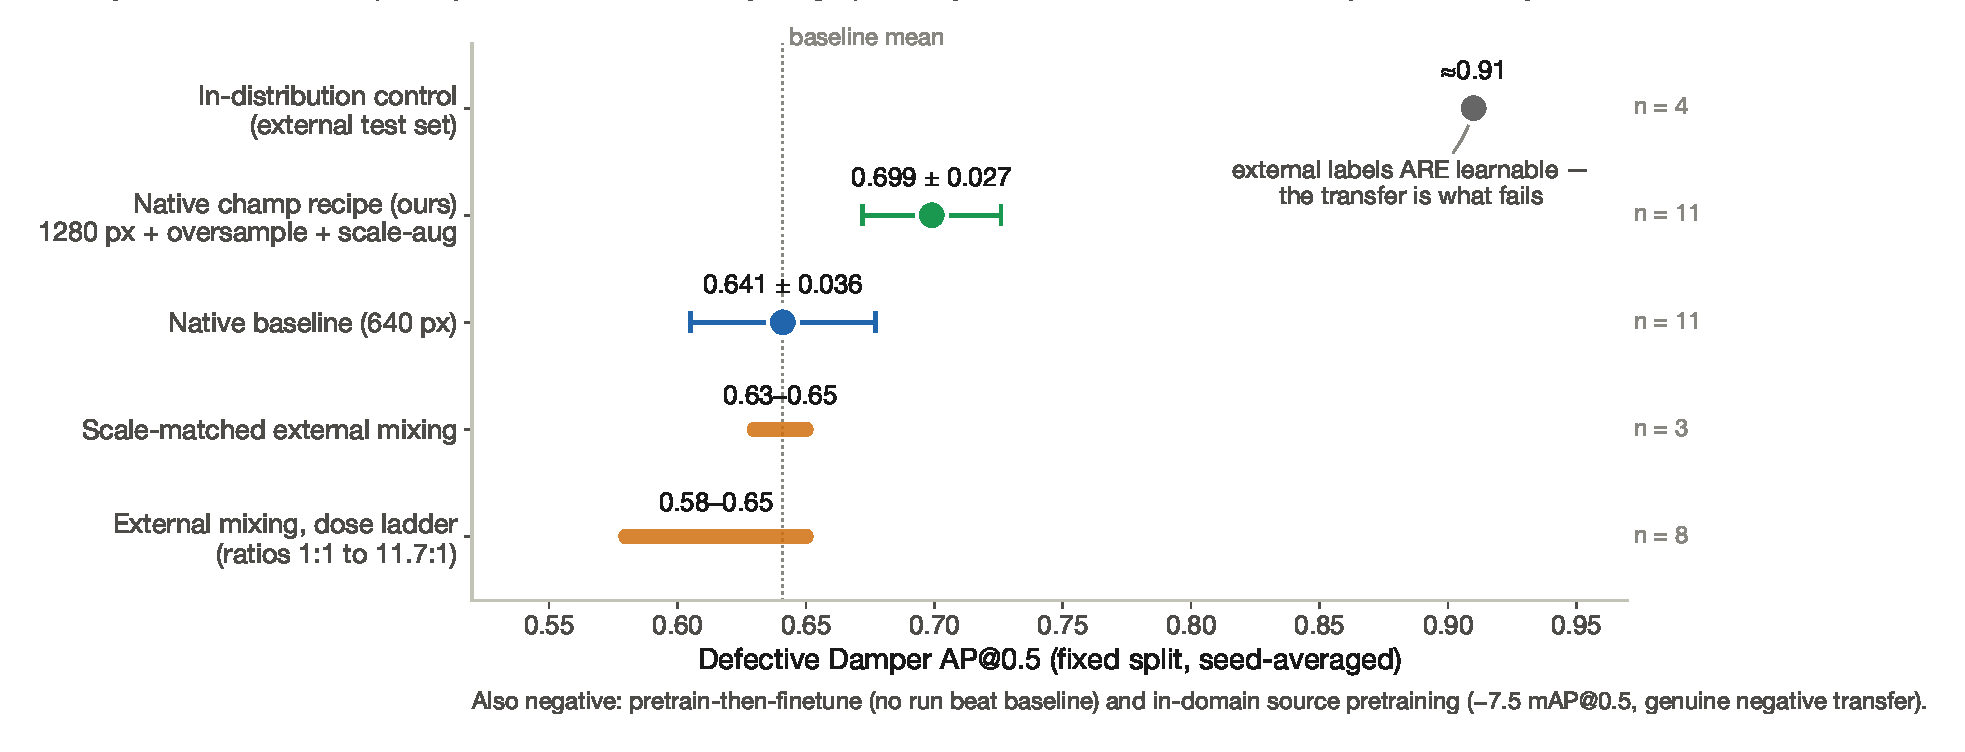
\includegraphics[width=0.82\textwidth]{figures/fig_external_paper.pdf}
%\caption{External-data routes vs.\ the native recipe on the earlier pool's fixed split (\dd{} AP@0.5, seed-averaged). No external route beats the native baseline; the in-distribution control shows the external labels are learnable---the transfer is what fails.}
%\label{fig:external}
%\end{figure*}

\subsection{Ablations and Negative Results}
\label{sec:ablations}
\textbf{Lighter backbones do not pay off.} Added to the rotation configuration, every backbone graft loses substantially at 1280\,px ($-7.6$ to $-11.1$ mAP for YOLO11n grafts, $-7.5$ to $-15.0$ for YOLOv8n grafts), the losses \emph{grow} at 640\,px (up to $-15.5$), and every YOLOv8n graft twin underperforms its YOLO11n counterpart (Fig.~\ref{fig:fpsfrontier} places the grid on the accuracy--throughput plane). The stride-4 P2 head also fails at 640\,px (68.2\% vs.\ 72.6\% for its stock twin), attributable to its freshly initialized head layers forfeiting part of the COCO initialization---worth noting because P2 heads are a standard small-object technique in aerial detection \cite{laf2026yolo}. In contrast with the group's wildfire study, where a Ghost-modified backbone traded ${\sim}8$ mAP points for a $4\times$ CPU speedup \cite{vazquez2026wildfire}, here the grafts' accuracy cost is not repaid in speed on GPU-class edge hardware (Section~\ref{sec:edge}), so the stock YOLO11n-OBB architecture dominates the entire graft frontier.

% "Other rejected techniques" paragraph removed from the paper (2026-09-10) —
% kept here as a comment for the GitHub record.
%\textbf{Other rejected techniques.} On the earlier pool's fixed split: freezing 10 backbone layers during fine-tuning costs $-5$ mAP and freezing 20 collapses training (44.8\%), confirming that full fine-tuning is required, in line with \cite{tsai2025atli} and opposite to classification-side practice \cite{shakiba2022insulator}; extending stage one to 300 epochs overfits the rare class and underperforms; test-time augmentation was worthless ($+0.2$ mAP). On the decontaminated 768\,px split, axis-aligned rotation of only $10^\circ$ costs $-10$ \dd{} AP points via box inflation. On the 974-image benchmark at 640\,px, three recall-recovery attempts---$6\times$ oversampling, doubling the classification-loss gain, and their combination---were flat or negative, as were multi-scale training and extended mosaic-free epochs. The pattern is consistent: once the data-centric recipe saturates, further training-side tweaks do not move the rare class; the remaining recall is threshold-limited, not model-limited (Section~\ref{sec:edge}).

\subsection{Resolution Scaling and Edge Deployment}
\label{sec:edge}
% NOTE: Soum (PhD student) will add further hardware analysis — additional
% platforms (e.g., Raspberry Pi) and how different models run on different
% hardware. Details in this subsection may be revised by that work.
Fig.~\ref{fig:resfrontier} plots the resolution frontier. Two deployment paths were compared at every inference resolution: retraining natively at the target resolution with the best 640-compatible recipe, and simply running a 1280-trained model at reduced inference resolution. The second path is nearly free: the 1280-trained mixup-recipe model evaluated at 640/768/960/1024\,px scores 73.2/76.5/78.8/79.8\% \map{} (80.4\% at native 1280), so inferring at 768 costs only ${\approx}4$ points and even edges out dedicated 768\,px retraining (75.1--76.3\%). The gap between 640-trained and 1280-trained models evaluated at the same 640\,px input is small (72.6\% vs.\ 73.2\%): the resolution gap is a test-time information loss, not a training deficiency, so one 1280-trained model can serve every deployment resolution. For deployments that must both train and infer at 640\,px, the blur+mixup+$30^\circ$ recipe transfers: 76.4\% \map{}, $+9.6$ points over the 640 baseline. Where screening recall matters more than precision, lowering the confidence threshold from 0.5 to 0.1 buys $+13$ points of defect recall at precision ${\approx}0.55$---the remaining misses are threshold-limited, not model-limited.

\begin{figure}[t]
\centering
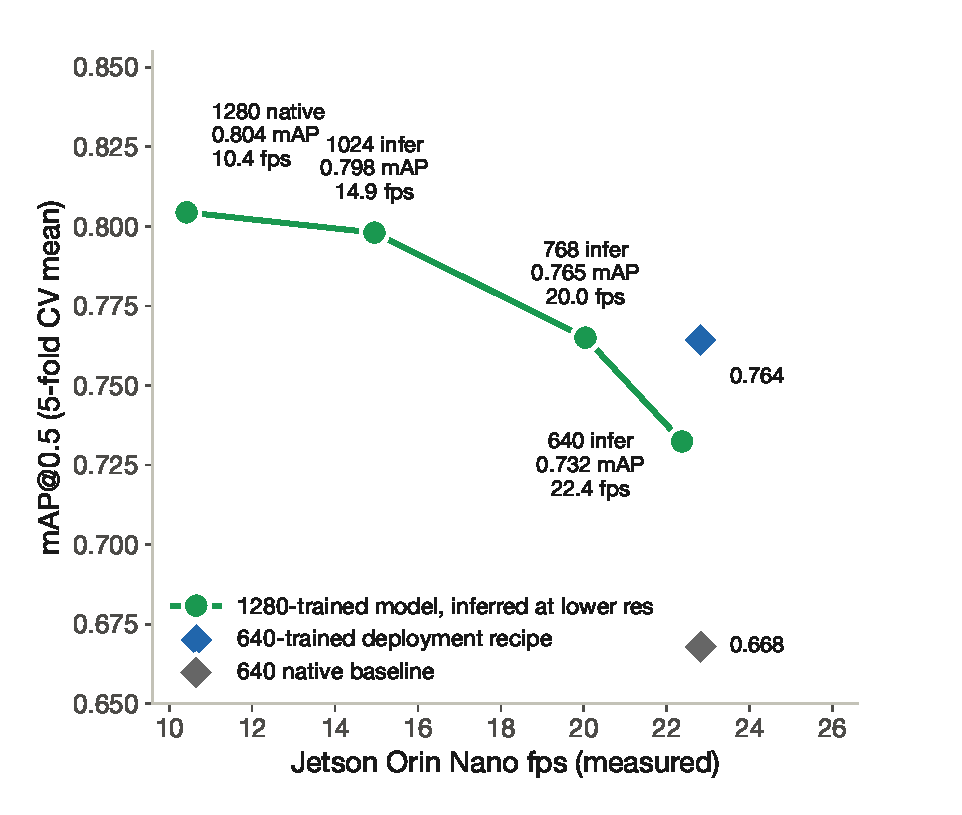
\includegraphics[width=\columnwidth]{figures/fig_resfrontier_paper.pdf}
\caption{Resolution frontier (5-fold means, measured Jetson Orin Nano throughput): the 1280-trained mixup-recipe model at reduced inference resolutions vs.\ 640-trained reference points (diamonds: 640 deployment recipe 76.4\%, 640 baseline 66.8\%).}
\label{fig:resfrontier}
\end{figure}

Table~\ref{tab:jetson} reports measured end-to-end throughput on the Jetson Orin Nano, and Fig.~\ref{fig:fpsfrontier} places the architecture grid on the accuracy--throughput plane. These results provide three key takeaways. First, TensorRT FP16 is the correct export: the architecture reaches \textbf{34.8 FPS} at 640\,px---above the 25--30 FPS real-time standard for drone footage \cite{vazquez2026wildfire} at 73--76\% \map{}---and 23.4 FPS at 768\,px, while even 1280\,px PyTorch inference (10.4 FPS, 82.0\% \map{}) satisfies the 5--10 FPS screening requirement; the export itself cost $-0.9$ mAP points when validated on the earlier campaign's 768\,px deployment retrain. Second, INT8 quantization is a documented negative result on this software stack: the INT8 engine is \emph{slower} than FP16 (30.1 vs.\ 34.8 FPS at 640\,px) and loses 10 \dd{} AP points (53.0\% vs.\ 62.8\%, $n{=}1$ fold)---the predicted minority-class quantization damage---so FP16 remains the deployment precision; preserving INT8 accuracy in inspection detectors has been reported to require quantization-aware training rather than the post-training calibration used here \cite{farooq2026teyolov8}. Lastly, the backbone grafts' theoretical FLOP savings do not convert to useful speed at matched accuracy (the Ghost graft's 45.9 FPS at 640\,px comes with a 15-point mAP deficit), and TensorRT is anomalously slower than PyTorch for some graft and high-resolution combinations on this early JetPack~7.2/TensorRT~11.1 stack; stock YOLO11n-OBB at 640--768\,px FP16 is the recommended operating point. All measurements were taken at the fixed 15\,W profile with clocks pinned; per-inference power draw and energy-delay product were not instrumented, unlike \cite{vazquez2026wildfire}, and are left for future work.

\begin{table}[t]
\caption{Measured end-to-end throughput (FPS, batch 1) of the YOLO11n-OBB architecture on the Jetson Orin Nano (15\,W, clocks pinned). \map{} column: the 1280-trained mixup-recipe model evaluated at each inference resolution (the final recipe reaches 82.0\% at 1280; its reduced-resolution probes were not run).}
\label{tab:jetson}
\centering
\scriptsize
\setlength{\tabcolsep}{4pt}
\begin{tabular}{lcccc}
\toprule
Input (px) & \map{} (\%) & PyTorch FP32 & TensorRT FP16 & TensorRT INT8 \\
\midrule
640 & 73.2 & 22.4 & \textbf{34.8} & 30.1 \\
768 & 76.5 & 20.0 & 23.4 & 21.7 \\
1024 & 79.8 & 15.0 & 11.9 & --- \\
1280 & 80.4 & 10.4 & 6.5 & --- \\
\bottomrule
\multicolumn{5}{l}{INT8 engines were not built at 1024/1280 after the 640/768}\\
\multicolumn{5}{l}{results showed INT8 dominated by FP16 in both speed and accuracy.}
\end{tabular}
\end{table}

\begin{figure}[t]
\centering
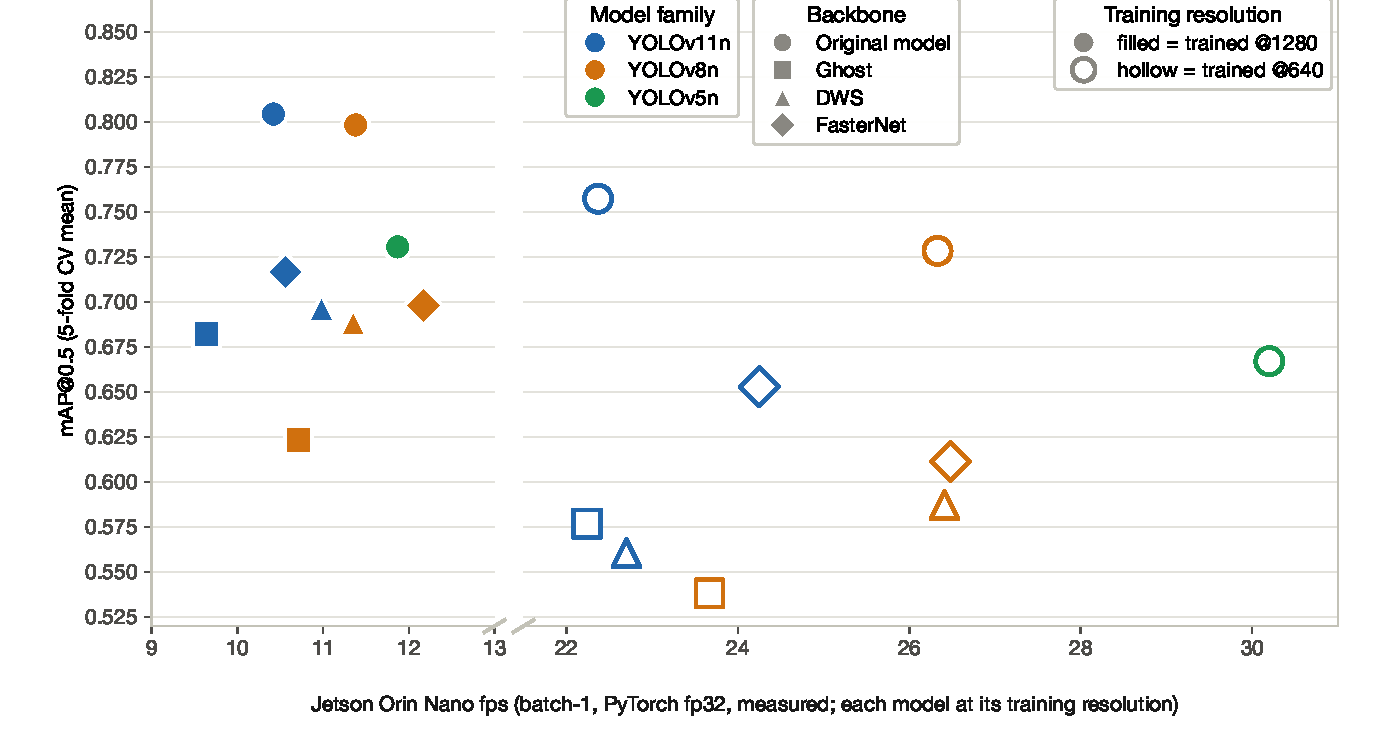
\includegraphics[width=\columnwidth]{figures/fig_fps_paper.pdf}
\caption{Accuracy vs.\ measured Jetson Orin Nano throughput across the model families and backbone grafts (filled: trained and deployed at 1280\,px; hollow: 640\,px). Stock YOLO11n-OBB dominates the backbone-graft frontier at matched throughput.}
\label{fig:fpsfrontier}
\end{figure}

% =====================================================================
\section{Conclusion}
\textit{[Placeholder --- suggested text, following the sample paper's convention.]} The key findings of this work are as follows:
\begin{enumerate}
\item A data-centric recipe---1280\,px training, $3\times$ defect oversampling, scale/rotation augmentation, OBB task mode, mixup, and blur augmentation---raises YOLO11n from 66.8\% to 82.0\% \map{} and nearly $+30$ \dd{} AP points on a decontaminated 974-image benchmark, with no new labels, no external data, and no architecture change.
\item The recipe ordering is architecture-independent across YOLOv5n, YOLOv8n, and YOLO11n, with YOLO11n leading at the strongest configurations, and the tuned 2.6M-parameter model matches a stock 47M-parameter DINO-4scale under identical cross-validation folds.
\item Every external-data route (mixing, curation, staged pretraining, in-domain source pretraining) failed on the rare class across all three architectures, while in-distribution controls prove the external labels learnable: what transfers is label-style consistency, not domain proximity.
\item Evaluation hygiene is a first-class problem on small benchmarks: three public datasets duplicate into the ATLI evaluation split, and single-split rare-class AP swings by more than 20 points across equally valid draws; cross-validated means behind a leakage gate are the minimum reporting standard.
\item Augmentation techniques hit a composition ceiling (CPLID restore, shear, and blur all fail to stack on the rotation configuration), but mixup composes, and blur+mixup jointly unlock a stronger rotation dose---the final recipe is an interaction effect.
\item The model runs in real time on a Jetson Orin Nano: 34.8 FPS at 640\,px with TensorRT FP16 (73--76\% \map{}), with 82.0\% \map{} available at 1280\,px at a screening-rate 6.5--10.4 FPS; INT8 is slower and damages the rare class on this stack, so FP16 is the deployment precision.
\end{enumerate}
Looking ahead, this research can be extended by applying the data-centric recipe to a heavyweight detector under a matched budget, instrumenting on-device power draw and energy-delay product, recovering INT8 through quantization-aware training, enlarging the defective-damper evaluation pool, and validating the deployed engine on in-flight video.

\bibliographystyle{IEEEtran}
\bibliography{refs,refs_extra,refs_new,refs_sota}

\end{document}
